\section{E. 시험자리 배정하기}

\begin{frame} % No title at first slide
    \sectiontitle{E}{시험자리 배정하기}
    \sectionmeta{
        \texttt{network\_flow}\\
        출제진 의도 -- \textbf{\color{acsilver}Medium}
    }
    \begin{itemize}
        \item 출제자: \texttt{riroan}
    \end{itemize}
\end{frame}

\begin{frame}{\textbf{E}. 시험자리 배정하기}

    \begin{itemize}
        \item 단순 방향 그래프 $G = (V, E)$, 두 정점 $S, E$, 각 정점별 비용 $C_v$, 자연수 $K \leq 5$
        \item 비용의 합이 최소이면서 다음의 조건을 만족하는 정점 집합 $X$를 찾는 것이 목표입니다.
        \item 조건: $S$에서 $E$로 가는 모든 경로들이 $X$의 원소를 적어도 $K$개 포함하는 것
    \end{itemize}
    
    \begin{center}
        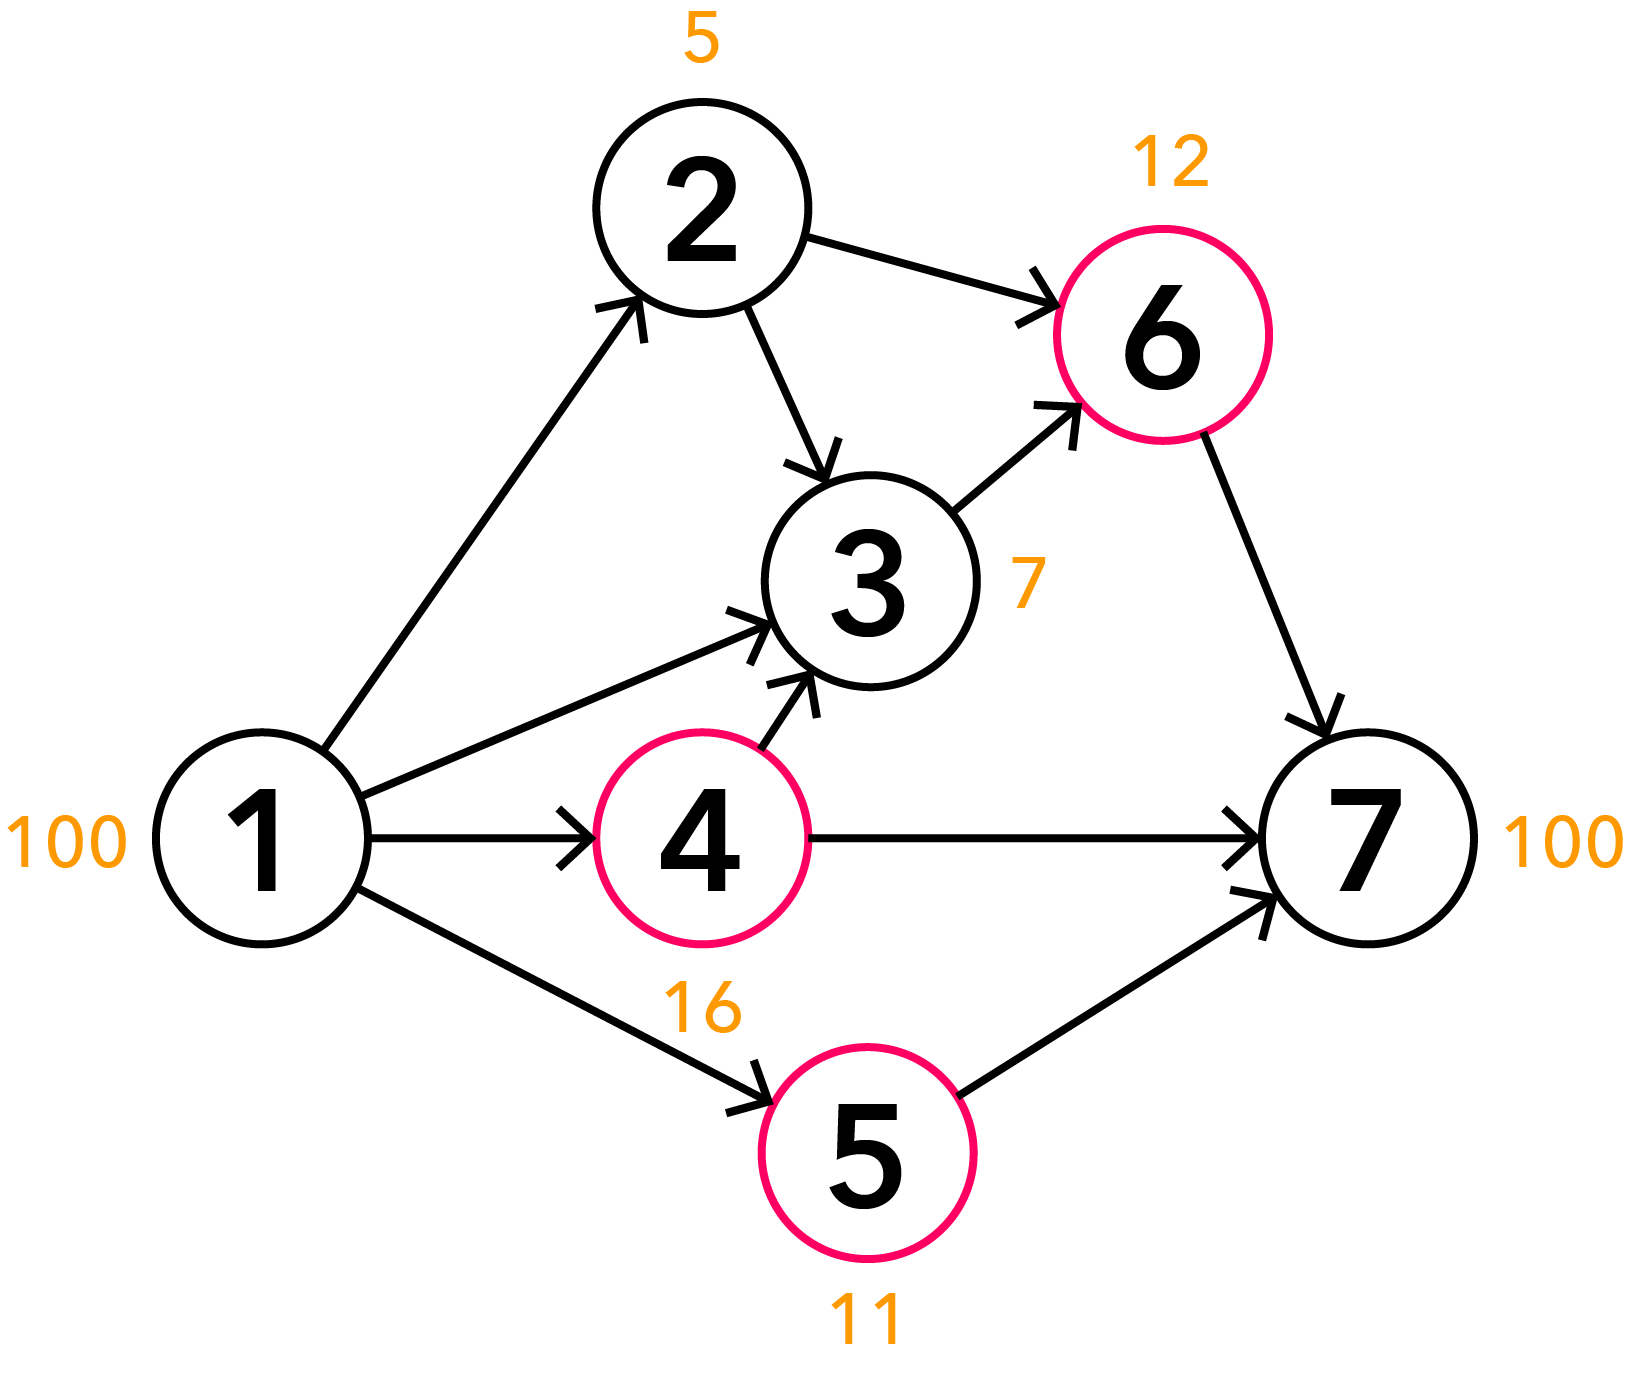
\includegraphics[width=0.3\linewidth]{../images/setting-maps/maps_ex_1.png}
    \end{center}
    
\end{frame}